\documentclass[acmsmall,screen,review]{acmart}

\setcopyright{none}
\settopmatter{printacmref=false}
\renewcommand\footnotetextcopyrightpermission[1]{}
\pagestyle{plain}

\acmJournal{CSUR}

\usepackage{booktabs}
\usepackage{tabularx}
\usepackage{multirow}
\usepackage{array}
\usepackage{longtable}
\usepackage{enumitem}
\usepackage{xspace}
\usepackage{graphicx}
\usepackage{hyperref}
\usepackage{microtype}
\usepackage{tikz}

\usetikzlibrary{arrows.meta,positioning}

\newcolumntype{Y}{>{\raggedright\arraybackslash}X}

\newcommand{\sysproblem}{state management in parallel and distributed systems\xspace}

\begin{document}

\title{Efficient State Management in Parallel and Distributed Systems}

\author{Shuhao Zhang}
\orcid{0000-0000-0000-0000}
\affiliation{%
  \institution{Huazhong University of Science and Technology}
  \city{Wuhan}
  \country{China}}
\email{shuhaozhang@hust.edu.cn}

\begin{abstract}
State has become the operational core of modern data systems. Stream processors, transactional streaming engines, edge analytics stacks, approximate execution runtimes, large language model serving systems with large key-value (KV) caches, retrieval-augmented generation services, and continual-learning systems all rely on shared, evolving, and performance-critical state. Yet the literature remains fragmented: one body of work studies contention-aware access paths, another focuses on hardware-conscious execution and multi-objective control, a third studies memory management and scheduling for LLM serving, and a fourth examines persistent updates, memory retention, and cross-round reuse for long-running intelligent services. This survey organizes these lines under a unified systems question: how can a parallel or distributed runtime keep state observable, schedulable, efficient, and reusable under complex hardware and dynamic workloads?

We structure the survey around three tightly coupled dimensions of state management. First, we review state access and scheduling, covering online observation, hotspot diagnosis, locality-aware cost modeling, and runtime control for shared state under concurrency. Second, we review state-aware execution optimization, focusing on how hardware topology, KV-cache memory management, energy constraints, latency-service objectives, approximation boundaries, and quality guarantees jointly shape end-to-end gains. Third, we review state evolution and reuse, covering online updates, continual retention, dynamic knowledge maintenance, and memory-centric inference pipelines. Across these dimensions, we highlight a common propagation effect: local mismatches in access, execution, or evolution often amplify into system-level instability.

Beyond summarizing the literature, the survey contributes a unifying conceptual framework, a cross-domain taxonomy, and an agenda for future systems that integrate access governance, execution control, and memory evolution into one runtime loop. We argue that the next generation of stateful infrastructure---especially for intelligent services on heterogeneous hardware---should treat state management not as a storage detail but as the central systems abstraction that links observability, control, and long-horizon service quality.
\end{abstract}

\keywords{stateful systems, stream processing, distributed systems, runtime optimization, heterogeneous hardware, LLM serving, KV cache, continual learning, retrieval-augmented generation}

\maketitle

\section{Introduction}

The dominant systems abstractions of the last decade have shifted from stateless throughput engines toward long-running services that continuously interact with state. Foundational streaming systems such as MillWheel, Naiad, D-Streams, and the Google Dataflow model already made state and time first-class runtime concerns~\cite{akidau2013millwheel,murray2013naiad,zaharia2013dstreams,akidau2015dataflow}. A transactional stream processor maintains window contents, indexes, queues, and recovery metadata~\cite{zhang2017revisiting,zhang2019briskstream,mao2023morphstream}. An edge analytics pipeline relies on compression dictionaries, approximate intermediate summaries, and quality-aware operator state~\cite{zeng2024cstream,zeng2024pecj}. An LLM serving runtime maintains per-request KV caches, page tables, prefix-sharing structures, and decode scheduling metadata that directly determine throughput and latency~\cite{kwon2023pagedattention,agrawal2024sarathi,zheng2023sglang}. A modern retrieval-augmented or continual-learning service maintains evolving memory, retriever parameters, retained samples, and update traces across rounds of inference~\cite{wu2023sentistream,zhou2025ferret,li2025global,zhang2026flowrag}. In all of these cases, system behavior depends less on the existence of state than on how that state is accessed, executed upon, updated, retained, and reused.

This evolution has made \sysproblem both more important and more difficult. Traditional decomposition often studies operator placement, memory layout, or model adaptation separately. In practice, these concerns interact. A hotspot in shared state access can change queueing behavior and hide locality opportunities. An optimization that improves kernel speed on one processor may fail to improve service-level latency once energy, data movement, or accuracy constraints are accounted for. A memory update rule that accepts more new information may destabilize retention, retrieval quality, or inference consistency downstream. The systems challenge is therefore not merely to optimize state in one phase, but to manage propagation across the full lifecycle of state.

This survey is motivated by that propagation view. We define state management as the set of mechanisms that govern how shared state is organized, observed, accessed, updated, retained, and reused across execution boundaries. Under this definition, state management spans classic streaming systems, hardware-conscious data processing, and newer AI runtimes. The common question is how to keep stateful execution stable, efficient, and controllable under concurrency, topology, and non-stationary workloads.

The propagation view also clarifies why the same systems pattern keeps reappearing across otherwise different domains. In a multicore streaming engine, the critical control variable may be a shared hash table, window buffer, or recovery log. In an edge analytics runtime, it may be a compression dictionary or bounded error-compensation state. In an LLM serving runtime, it may be the KV cache together with the allocator, page table, prefix tree, or reuse index that governs who can touch it and when~\cite{kwon2023pagedattention,zheng2023sglang}. In a retrieval-augmented service, it may be a retriever memory, vector index, or retained coreset. The concrete state object changes, but the systems obligations do not: make the object visible to the runtime, characterize its access cost, couple it to execution policy, and ensure that updates do not destroy its future reuse value.

Our synthesis is organized around three dimensions:

\begin{enumerate}[leftmargin=*]
\item \textbf{State access and scheduling}: how systems expose contention, model access cost, and schedule work around hotspots, topology, and recovery requirements.
\item \textbf{State-aware execution optimization}: how systems turn state layout and execution coupling into stable end-to-end gains under hardware, energy, latency, and quality constraints.
\item \textbf{State evolution and reuse}: how systems continuously write, retain, organize, and reuse state for dynamic learning and inference.
\end{enumerate}

Figure~\ref{fig:propagation} summarizes the organizing perspective used throughout the survey. Rather than viewing access, execution, and evolution as independent stages owned by different subsystems, we treat them as a single control loop over long-lived state. That framing matters for survey methodology as well: a result counts as state-management progress only if it explains a control decision over that loop, not merely a one-off local acceleration.

The survey makes three concrete contributions. First, it offers a unified vocabulary that connects streaming, approximate execution, and memory-centric intelligent services. Second, it proposes a taxonomy that separates state problems by \emph{access}, \emph{execution}, and \emph{evolution} while emphasizing their feedback loops. Third, it identifies a research agenda for integrated runtimes that coordinate state observability, scheduling, update control, and reusable memory services on heterogeneous hardware.

\begin{figure*}[t]
\centering
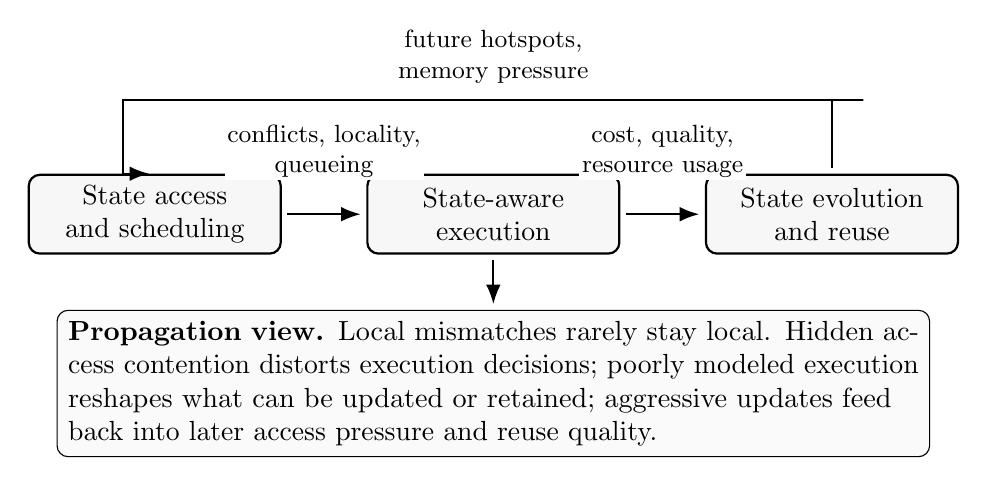
\begin{tikzpicture}[
  box/.style={draw, rounded corners, thick, align=center, minimum width=32mm, minimum height=10mm, fill=black!3},
  note/.style={draw, rounded corners, align=left, inner sep=4pt, fill=black!2},
  labelnote/.style={align=center, fill=white, inner sep=1pt, font=\small},
  arrow/.style={-{Latex[length=2.5mm]}, thick, shorten <=2pt, shorten >=2pt}
]
\node[box] (access) at (0,0) {State access\\and scheduling};
\node[box] (exec) at (4.3,0) {State-aware\\execution};
\node[box] (evo) at (8.6,0) {State evolution\\and reuse};
\node[labelnote] (l1) at (2.15,0.8) {conflicts, locality,\\queueing};
\node[labelnote] (l2) at (6.45,0.8) {cost, quality,\\resource usage};
\node[labelnote] (fb) at (4.3,2.0) {future hotspots,\\memory pressure};
\node[note, text width=108mm] (note1) at (4.3,-2.15) {
\textbf{Propagation view.} Local mismatches rarely stay local. Hidden access contention distorts execution decisions; poorly modeled execution reshapes what can be updated or retained; aggressive updates feed back into later access pressure and reuse quality.
};

\coordinate (topL) at (-0.4,1.45);
\coordinate (topR) at (9.0,1.45);

\draw[arrow] (access.east) -- (exec.west);
\draw[arrow] (exec.east) -- (evo.west);
\draw[arrow] (evo.north) |- (topR) -- (topL) |- (access.north);
\draw[arrow] (exec.south) -- (note1.north);
\end{tikzpicture}

\caption{A propagation-oriented view of state management. The survey's core claim is that access, execution, and evolution are coupled through feedback rather than separable pipeline stages.}
\label{fig:propagation}
\end{figure*}

\section{Foundations: Scope, Model, and Taxonomy}

We focus on systems in which state is both shared and performance-critical. This includes stream processing engines, transactional streaming systems, edge and heterogeneous analytics runtimes, approximate execution frameworks with quality constraints, and dynamic AI services such as continual learning and retrieval-augmented generation. We exclude purely static database storage engines, purely model-centric training methods that do not expose runtime state-management mechanisms, and application papers where state is incidental rather than central.

Our source material combines representative systems papers, journal articles, and recent intelligent-service systems papers. The initial seed comes from a coherent line of work on shared-state access, hardware-conscious execution, and evolving memory-centric services~\cite{zhang2024survey,zhang2020hardware,mao2023morphstream,wu2023sentistream,zhang2026flowrag}. We extend outward to include the broader systems context needed to interpret these results, including foundational streaming systems~\cite{akidau2013millwheel,murray2013naiad,zaharia2013dstreams,akidau2015dataflow}, stateful serving runtimes for LLM inference~\cite{kwon2023pagedattention,agrawal2024sarathi,zheng2023sglang}, recovery systems, compression and approximation frameworks, and dynamic retrieval services. The resulting survey should be read as a systems synthesis rather than a bibliometric catalog or a lineage-specific retrospective.

We use three inclusion criteria. First, the system must surface state as an explicit runtime concern rather than a hidden storage detail. Second, the paper must expose a systems mechanism such as scheduling, cost modeling, update control, migration, retention, or reuse orchestration. Third, the evaluation must connect that mechanism to end-to-end properties such as throughput, tail latency, recovery time, quality degradation, or long-horizon reuse quality. These criteria intentionally bias the survey toward papers that make control decisions legible. They also explain why some influential application papers appear only as context: many use state, but fewer reveal state management as the main systems abstraction.

\subsection{Broader Literature Landscape}

The broader systems literature suggests that efficient state management has never belonged to a single subcommunity. Early stream and event systems already exposed state placement, operator mobility, and recovery as central runtime problems, even when the terminology was not yet standardized. Aurora and Borealis made operator state explicit in continuous query plans; IBM InfoSphere Streams, Storm, Heron, and Flink pushed those ideas into large-scale deployments; Trill, Structured Streaming, Differential Dataflow, StreamCloud, and SABER showed that incremental maintenance, elasticity, and hardware-aware execution all reshape the state boundary itself; and surveys on stream processing and complex event processing documented how broad this design space had already become before today's AI-service wave~\cite{abadi2003aurora,abadi2005borealis,gedik2008infosphere,toshniwal2014storm,kulkarni2015heron,carbone2015flink,carbone2015asynchronous,chandramouli2014trill,armbrust2018structured,murray2013differential,nasir2019megaphone,gulisano2012streamcloud,koliousis2016saber,hirzel2014catalog,cugola2012processing}. What changes in modern deployments is less the existence of state than the heterogeneity and speed of the control loop around it.

An adjacent line of work came from transactional, replicated, and memory-resident data systems. H-Store, Spanner, Calvin, RAMCloud, FaRM, and later high-performance concurrency-control systems such as DrTM+H, TicToc, and NAM-DB treated state as a jointly managed object spanning consistency, placement, logging, and remote access. Classic snapshot and state-machine-replication results remain relevant here because they clarify a point that also matters for streaming and LLM serving: state is not only a performance artifact, but also a correctness boundary that constrains what can be migrated, replayed, or shared without breaking service guarantees~\cite{kallman2008hstore,corbett2012spanner,thomson2012calvin,ousterhout2011ramcloud,dragojevic2014farm,ren2015drtmh,yu2016tictoc,zamanian2017endmyth,schneider1990state,chandy1985snapshot,ongaro2014raft}. This broader context helps prevent a narrow reading in which state management is reduced to caching alone.

Model serving added another crucial perspective: once services must meet latency targets under bursty demand, state becomes the hidden scheduler for the whole runtime. Clipper established an early modular serving architecture in which caching, batching, and adaptive model selection are explicit runtime controls rather than framework internals~\cite{crankshaw2017clipper}. Clockwork sharpened that line by arguing that inference latency is predictable enough to support principled scheduling and strong request-level isolation, turning execution-time prediction into a state-aware admission and dispatch mechanism~\cite{gujarati2020clockwork}. More recent LLM-serving systems then made the coupling between scheduler structure and reusable inference state even more explicit through KV pages, LoRA adapter state, phase splitting, disaggregated prefill/decode paths, and prompt-generation composition strategies~\cite{shen2019nexus,crankshaw2020inferline,romero2021infaas,yu2022orca,sheng2023flexgen,li2023alpaserve,chen2024punica,kwon2023pagedattention,zheng2023sglang,agrawal2024sarathi,zhong2024distserve,patel2024splitwise,holmes2024fastgen}. From the survey's perspective, these papers matter not just because they accelerate inference, but because they expose short-lived memory objects as first-class scheduling and admission surfaces.

The literature on memory-augmented language models and retrieval systems broadens the time horizon of the problem. Transformer-XL and Compressive Transformer introduced explicit recurrent memory paths; kNN-LM, REALM, and RAG made external retrieval part of the inference loop; RETRO and Atlas showed how extremely large external memories can be operationalized; and newer systems such as LongMem, Self-RAG, HippoRAG, and RAPTOR push toward persistent, structured, and self-reflective memory layers that must be updated while queries continue to arrive~\cite{dai2019transformerxl,rae2020compressive,khandelwal2020knnlm,guu2020realm,lewis2020rag,wu2022memorizing,borgeaud2022retro,izacard2022atlas,wang2023longmem,asai2024selfrag,wang2024hipporag,sarthi2024raptor}. These systems reinforce the argument that KV caches are only one point in a larger design space of runtime-managed model state.

Continual learning and approximate data systems add yet another useful contrast. Experience-retention mechanisms such as EWC, GEM, iCaRL, A-GEM, replay-based methods, MIR, DER, REMIND, and GDumb study how bounded memory changes future model quality under online updates, while surveys in that area formalize retention and forgetting as explicit systems constraints~\cite{kirkpatrick2017ewc,lopez2017gem,rebuffi2017icarl,chaudhry2019agem,rolnick2019experience,aljundi2019mir,buzzega2020der,hayes2020remind,prabhu2020gdumb,delange2021survey}. In parallel, BlinkDB, ApproxHadoop, ApproxJoin, StreamApprox, and IncApprox show that large-scale analytics systems already learned a complementary lesson: once stateful summaries or samples are used to save work, the runtime must jointly control error, update cost, and future reuse value~\cite{agarwal2013blinkdb,goiri2015approxhadoop,wang2018approxjoin,hu2018streamapprox,chen2018incapprox}. Taken together, these lines of work justify the broad stance of this survey: efficient state management is a shared systems problem that cuts across streams, storage, serving, retrieval, and learning.

General-purpose dataflow and storage systems provide another part of the same genealogy. Dryad, FlumeJava, and CIEL helped establish distributed dataflow as a programmable runtime substrate rather than a fixed relational engine, while Bigtable, Dynamo, Cassandra, Megastore, and Percolator clarified how large-scale services externalize state into replicated, incrementally updated storage layers with explicit consistency and update semantics~\cite{isard2007dryad,chambers2010flumejava,murray2011ciel,chang2008bigtable,decandia2007dynamo,lakshman2010cassandra,baker2011megastore,peng2010percolator}. Stream systems later pulled these concerns back into low-latency pipelines through SEEP and operator-state-management work that treated elasticity and fault tolerance as state redistribution problems rather than mere operator replication~\cite{fernandez2010seep,fernandez2013osm}. At the same time, replicated-data abstractions such as CRDTs and retrieval-side structures such as dense passage indexes, late-interaction retrievers, product quantization, and HNSW graphs show that modern memory layers increasingly combine distributed-systems semantics with machine-learning retrieval paths~\cite{shapiro2011crdt,karpukhin2020dpr,khattab2020colbert,jegou2011pq,malkov2020hnsw}. Even low-level attention kernels belong in this picture: implementations such as FlashAttention-2 determine when attention state can stay on-chip, when it must be materialized, and how memory traffic constrains serving-scale state management~\cite{dao2024flashattention2}.

\subsection{A Unifying View of Stateful Computing Systems}

\subsubsection{What Counts as State?}

In this survey, \emph{state} includes any persistent or semi-persistent runtime object whose value influences future execution beyond a single operator invocation. Examples include hash tables and windows in streaming operators, shared indexes and queues in multicore runtimes, compression dictionaries, adaptive buffering metadata, KV caches and their page-allocation metadata in LLM serving systems, coresets for continual learning, retriever memory, and structured knowledge stores used by intelligent services. This definition intentionally spans in-memory, persistent, and hybrid forms of state.

Two properties make state systems-hard. First, state is usually shared across tasks, requests, or time windows, so access conflicts propagate. Second, state is temporally extended: the way a system updates state today changes tomorrow's optimization space. These properties mean that local decisions often have delayed and cross-layer consequences.

\subsubsection{The Propagation Perspective}

We organize \sysproblem using a propagation perspective. Figure design is left for later revision, but the conceptual pipeline is straightforward. A request first encounters \emph{state access}: it must find, read, or synchronize on shared state. The resulting data path determines \emph{state-aware execution}: work is mapped to cores, sockets, accelerators, or approximate operators subject to latency and quality goals. The outputs then contribute to \emph{state evolution}: some state is updated, some is retained, and some is exposed for future reuse. Failures or mismatches in any stage propagate. Uncontrolled contention in access may destroy locality and distort execution modeling. Mis-modeled execution trade-offs may make update policies unsustainable. Over-aggressive updates may increase access pressure and destabilize future inference.

This view differs from traditional layered designs that isolate storage, scheduling, and adaptation. The literature repeatedly shows that state problems cross those layers. Shared access depends on topology-aware execution~\cite{zhang2019briskstream,zhang2020concurrent}. Quality-aware execution depends on error-aware state evolution~\cite{zeng2024pecj}. Continual memory reuse depends on stable update and retention mechanisms~\cite{zhou2025ferret,li2026streamfp,zhang2026flowrag}. The propagation perspective therefore provides a more faithful abstraction for long-running stateful systems.

\subsection{Taxonomy of State Management Problems}

Table~\ref{tab:taxonomy} summarizes the taxonomy used throughout the survey.

\begin{table*}[t]
\small
\caption{Taxonomy of state-management problems.}
\label{tab:taxonomy}
\begin{tabularx}{\textwidth}{>{\raggedright\arraybackslash}p{0.18\textwidth}YY}
\toprule
Dimension & Core question & Representative concerns \\
\midrule
Access and scheduling & How is shared state exposed, costed, and scheduled under concurrency? & hotspot diagnosis, conflict propagation, locality, topology, recovery, migration, prefix-aware sharing \\

Execution optimization & How does state interact with hardware and service objectives? & placement, compression, KV-cache paging, prefill/decode coupling, approximation, latency-energy-quality trade-offs \\

Evolution and reuse & How is state updated, retained, and reused over time? & online updates, memory budgets, cache growth and reclamation, sample selection, retriever drift, knowledge maintenance \\
\bottomrule
\end{tabularx}
\end{table*}

The taxonomy is intentionally operational. It does not classify systems by application domain but by the control problem they solve. A stream engine and a RAG service may both belong to the evolution-and-reuse category if the dominant challenge is continuous state updates and future reuse. Likewise, a compression engine and a transactional stream processor may both belong to execution optimization if the central problem is coordinating stateful execution with hardware constraints.

This taxonomy is useful precisely because it is not mutually exclusive at the whole-system level. Mature systems typically occupy more than one row of Table~\ref{tab:taxonomy}. A transactional stream engine may begin as an access-and-scheduling problem and grow into an execution-control problem once topology and recovery costs are modeled explicitly. A retrieval service may begin as an evolution-and-reuse problem but quickly become an access problem when vector indexes, retriever memories, and hot prompts create concentrated contention. The taxonomy should therefore be read as a decomposition of control surfaces, not as a rigid partition of system classes.

\subsubsection{A Reusable Analysis Scaffold}

To keep the rest of the survey cumulative rather than anecdotal, we use the same five-question scaffold whenever we summarize a system line. First, what is the \emph{state object}? Second, what \emph{control surface} does the runtime expose over that state, such as placement, scheduling, migration, admission, retention, or reuse? Third, what \emph{coupling path} makes that control surface important, for example contention, topology, phase asymmetry, drift, or quality decay? Fourth, what \emph{evaluation boundary} does the paper actually optimize, such as throughput, tail latency, recovery time, bounded error, or long-horizon reuse quality? Fifth, what \emph{remaining systems gap} is left open after the paper's mechanism is accounted for?

This scaffold matters for two reasons. It gives the survey a stable comparison unit across otherwise different domains, and it helps prevent a common failure mode in survey writing: turning papers into disconnected summaries of implementation details. Under this template, a stream processor, an LLM-serving runtime, and a retrieval-memory system can all be compared in terms of the state they expose, the runtime decision they support, the service boundary they optimize, and the control gap they leave unresolved.

\begin{table*}[t]
\small
\caption{Reusable analysis scaffold for extending the survey.}
\label{tab:scaffold}
\begin{tabularx}{\textwidth}{>{\raggedright\arraybackslash}p{0.18\textwidth}YY}
\toprule
Question & What to extract from each paper & Typical answers in this survey \\
\midrule
State object & Which runtime object persists across tasks, requests, or time? & windows, indexes, logs, dictionaries, KV caches, retriever memories, coresets \\

Control surface & What decision does the system make over that object? & placement, batching, migration, paging, admission, retention, reuse orchestration \\

Coupling path & Why does this state decision propagate to end-to-end behavior? & contention, locality, memory pressure, phase asymmetry, drift, quality-loss amplification \\

Evaluation boundary & Which system-level property is optimized or bounded? & throughput, p99 latency, recovery time, energy, bounded error, forgetting, reuse quality \\

Remaining gap & What is still missing after the paper's contribution? & weak observability, no closed loop, limited portability, incomplete lifecycle control, no long-horizon evaluation \\
\bottomrule
\end{tabularx}
\end{table*}

\subsubsection{Representative System Classes}

The state-management lens cuts across at least five recurring system classes. The first is \emph{high-throughput streaming and transactional dataflow}, where state appears as windows, per-key aggregates, dependency graphs, and recovery metadata. The second is \emph{hardware-conscious analytics}, where state appears as compressed representations, scheduling metadata, and approximation structures whose access pattern determines whether hardware speedups survive end-to-end execution. The third is \emph{LLM serving and memory-bound inference}, where state appears as KV caches, page tables, prefix-sharing structures, and structured decoding metadata that must be scheduled under tight memory and latency budgets~\cite{kwon2023pagedattention,agrawal2024sarathi,zheng2023sglang}. The fourth is \emph{continual learning and adaptive services}, where retained samples, coresets, and update traces define both learning cost and future accuracy. The fifth is \emph{memory-centric retrieval and agentic inference}, where retrievers, knowledge structures, and evolving indexes mediate multi-round reuse.

These classes matter because they expose different failure modes. Streaming systems fail by contention amplification, migration cost, or slow recovery. Hardware-conscious analytics fail by misplacing state relative to device topology or by violating quality boundaries when using approximate methods. LLM serving systems fail when KV-cache growth, fragmentation, or prefix-sharing policy turns memory into the primary throughput bottleneck. Continual-learning systems fail by exhausting budgets or forgetting useful history. Memory-centric inference systems fail by update drift, unstable retrieval, or uncontrolled growth in reusable state. A useful survey should make these failure modes comparable, because the same runtime ideas often reappear under different names.

\section{Core Dimensions of State Management}

\subsection{State Access and Scheduling}

\subsubsection{From Invisible Contention to Observable State Access}

Early multicore stream-processing work showed that poor performance often stemmed not from operator logic itself but from hidden contention in shared access paths. Revisiting stream-processing design on multicore processors demonstrated that shared queues, synchronization patterns, and fine-grained operator interactions could fundamentally limit scalability~\cite{zhang2017revisiting}. In parallel, multi-query optimization for complex event processing showed that sharing sub-computation is only beneficial when execution paths are carefully reorganized; otherwise, shared state can magnify interference rather than reduce work~\cite{zhang2017mqo}.

This line of work established a first principle: state management begins with observability. Systems need path-level metrics that connect hotspots, conflict density, queue growth, and throughput variation. Without such observability, tuning remains heuristic. This insight anticipated later systems that expose state access explicitly rather than burying it inside operator implementations.

\subsubsection{Cost Modeling Under Locality and Topology}

Once access patterns become observable, the next challenge is modeling their cost. BriskStream demonstrated that state hotspots and NUMA topology must be considered jointly; access-locality decisions that ignore topology can erase the gains of parallelization~\cite{zhang2019briskstream}. Subsequent work on concurrent stateful stream processing further showed that synchronization design, state partitioning, and task assignment must be analyzed together rather than in isolation~\cite{zhang2020concurrent}.

These results connect state management to a broader systems theme: locality is not a static placement problem, but a property created jointly by state layout, scheduling, and workload structure. Similar lessons appear in other stateful systems, including unified migration for distributed streaming~\cite{mao2025spacker} and online interval join systems where shared indexes and ordering constraints interact with runtime concurrency~\cite{zhang2023openmldb}. Across these works, the dominant abstraction is no longer simply a data structure. It is an access-cost surface shaped by contention and hardware placement.

\subsubsection{Runtime Control, Recovery, and Stateful Governance}

The mature form of access management is runtime control. MorphStream is representative: it treats transactional stream processing as a scheduling problem over stateful dependencies, allowing the engine to adapt execution plans at runtime rather than rely on fixed static policies~\cite{mao2023morphstream}. Follow-up work on fast parallel recovery shows that recovery must be integrated with steady-state execution rather than treated as a separate subsystem~\cite{zhao2024recovery}. Recovery metadata, log structure, and access control together determine whether a stateful engine can remain efficient after failures.

Earlier elasticity work makes the same point from another angle. SEEP framed elastic event processing as a problem of carrying operator state safely across a changing execution graph, while later operator-state-management work argued that scale-out and fault tolerance should share the same state-transfer machinery rather than be handled by unrelated control paths~\cite{fernandez2010seep,fernandez2013osm}. That lesson remains important today: if migration, checkpointing, and rescaling each maintain their own notion of state ownership, the runtime pays coordination cost repeatedly and recovery semantics become harder to reason about. A stronger design is to treat operator state as a first-class runtime object whose placement, replication, and transfer rules are reused across elasticity and fault handling.

The broader lesson is that access governance must eventually become a closed loop. Observation feeds cost modeling, which informs scheduling and recovery, which in turn changes future observation. This observation-model-control loop is one of the most reusable patterns in stateful systems research.

What distinguishes the strongest systems in this category is that they stop treating state access as an implementation detail. Once state becomes a scheduling object, new design options open up: conflict-aware batching, topology-sensitive placement, dependency-ordered execution, and recovery plans that are derived from steady-state access structure rather than bolted on afterward. This change in abstraction is at least as important as any single algorithmic optimization.

\subsubsection{Open Challenges in Access Management}

Despite the progress, at least four challenges remain. First, most systems still rely on coarse observability and do not expose state conflicts as first-class runtime objects. Second, topology-aware models often assume relatively stable hardware and workload structure. Third, recovery and migration are still commonly optimized separately from regular access control. Fourth, intelligent-service runtimes increasingly create new shared-state objects, such as vector indexes, retriever caches, and prefix-shared KV caches, whose conflict patterns are poorly understood. Future work should therefore extend access modeling to state objects that are semantic, dynamic, and cross-request.

\subsection{State-Aware Execution Optimization}

\subsubsection{Why Faster Kernels Do Not Guarantee Better Services}

A recurring mistake in systems design is to treat stateful execution as equivalent to faster kernels or better operator throughput. The literature reviewed here suggests a more nuanced picture. Once state interacts with heterogeneous hardware, moving data and coordinating access frequently dominate raw compute speed. Moreover, service objectives introduce latency, energy, and quality boundaries that can overturn microbenchmark gains.

FineStream provides a clear example. By studying fine-grained window-based stream processing on integrated CPU-GPU architectures, it showed that topology and data path design directly alter the feasible performance envelope~\cite{zhang2020finestream}. Co-running studies on integrated architectures made similar points from a broader resource-sharing angle~\cite{zhang2016corun,zhang2016elastic}. These systems emphasize that execution gains emerge only when state organization, data movement, and device mapping are optimized together.

\subsubsection{Energy, Compression, and Stateful Data Paths}

The CStream line deepens this theme by examining stateful compression on edge and asymmetric multicore devices~\cite{zeng2023cstreamicde,zeng2024cstream}. Compression dictionaries are state; their access pattern, update granularity, and task decomposition shape both energy and latency outcomes. The key finding is not merely that hardware-conscious compression helps, but that stateful compression creates a multi-objective problem spanning throughput, delay, energy, and compression ratio.

This observation generalizes beyond compression. Whenever the system carries intermediate state across operators or requests, execution policy becomes a question of which state transitions are affordable on the current hardware path. Device selection, data movement, and representation choice are therefore best viewed as one coupled decision rather than three independent knobs. The same principle is likely to matter even more for modern accelerator-rich inference deployments, where the cost of moving reusable state can dominate the cost of re-executing a kernel.

\subsubsection{KV-Cache Management as a State-Execution Problem}

Large language model serving makes this point unusually concrete. In these systems, the KV cache is not a minor implementation artifact. It is the dominant short-lived runtime state that grows with prompt length and output length, mediates prefix reuse, and constrains feasible batch size. vLLM made this explicit by treating KV-cache memory as a paged state object whose allocation and sharing policy determines whether throughput is limited by fragmentation, redundant duplication, and memory waste rather than raw compute; its central claim is that near-zero-waste allocation can directly enlarge feasible batch size and thereby raise throughput~\cite{kwon2023pagedattention}. Sarathi-Serve showed that the serving scheduler must also reason about the temporal evolution of that state, because prefill and decode phases create asymmetric pressure on the active cache footprint and therefore on latency-throughput trade-offs~\cite{agrawal2024sarathi}. SGLang extends the same theme to structured programs, where RadixAttention and compressed finite-state-machine decoding turn prompt overlap and output constraints into runtime-managed state-sharing and decoding-control opportunities~\cite{zheng2023sglang}. DeepSpeed-FastGen adds a complementary perspective: prompt and generation phases can be fused and split dynamically to improve throughput and reduce average and tail latency for long-prompt workloads, which again shows that serving policy is ultimately a policy over evolving short-lived state rather than over compute kernels alone~\cite{holmes2024fastgen}.

Read together, these papers also clarify a historical progression in serving infrastructure. Clipper treated serving as an orchestration layer over caching, batching, and model choice; Clockwork emphasized predictability and performance isolation; vLLM reframed memory allocation itself as the bottlenecked state plane; and SGLang plus FastGen showed that once requests become structured or long-context, the runtime must additionally optimize reuse boundaries across multi-call programs and prompt-generation phase transitions~\cite{crankshaw2017clipper,gujarati2020clockwork,kwon2023pagedattention,zheng2023sglang,holmes2024fastgen}. That progression is precisely why KV-cache management belongs inside a broader state-management survey rather than in a narrow inference-kernel discussion.

These systems support the broader claim of this survey: KV-cache management is a state-management problem. The cache persists across token steps, affects future scheduling decisions, exposes a reuse surface across requests, and demands explicit policies for allocation, sharing, reclamation, and placement. Once stated this way, KV-cache paging, prefix reuse, and decode scheduling sit naturally beside window management, dictionary placement, and retriever maintenance as instances of the same systems abstraction.

Closely related work on compressed stream processing without decompression and data-aware adaptive compression extends this view to database-style execution~\cite{zhang2023compressstreamdb,yu2025adaptivecompression}. Here, state-aware execution means choosing representation, operator placement, and access path jointly. The system's real unit of optimization becomes a stateful data path rather than an isolated operator.

\subsubsection{Approximation and Quality Boundaries}

Approximate execution adds another layer: the system must reason not only about cost but also about output quality. PECJ addresses disorder in stream window joins by proactively compensating for missing or late data using explicit error modeling~\cite{zeng2024pecj}. LibAMM studies approximate matrix multiplication and shows that algorithm choice, dataset properties, and memory behavior jointly determine whether approximate computing yields a stable efficiency-accuracy trade-off~\cite{zeng2024libamm}. Adaptive sampling systems for joins and video databases reach similar conclusions: approximation is useful only when quantity, quality, and system cost are modeled together~\cite{tang2025freesam,xu2024leap}.

These works suggest a generalized principle for state-aware execution. When intermediate or retained state influences correctness, one must model an \emph{execution boundary} rather than a single performance target. This boundary is defined by hardware topology, state access cost, and quality tolerance. Stable gains occur only within a limited operating region.

\subsubsection{Toward Closed-Loop Execution Control}

The next step is to unify these mechanisms into online control loops. Existing systems have already established many ingredients: topology-aware mapping~\cite{zhang2020finestream}, energy-aware decomposition~\cite{zeng2024cstream}, and quality-aware compensation~\cite{zeng2024pecj}. What remains comparatively underdeveloped is an integrated runtime that combines state observability with online execution control across heterogeneous processors and service objectives. This gap is particularly important for modern inference stacks, where accelerator choice, memory transfer, approximation, and retrieval quality all interact.

\subsection{State Evolution and Reuse}

\subsubsection{From Updates to Long-Horizon Memory}

The third major dimension of \sysproblem concerns what happens after execution produces new information. In many older data systems, state updates were treated as maintenance. In dynamic AI services, updates are themselves central: the system must decide what to absorb, what to retain, what to discard, and how to expose retained state for future reuse.

SentiStream is illustrative. It frames adaptive online sentiment analysis as a co-training problem over evolving data streams, effectively making model adaptation and runtime update part of the same loop~\cite{wu2023sentistream}. MOStream similarly treats data stream clustering as a modular, self-optimizing problem where summarization, windowing, refinement, and outlier control determine whether the system can keep up with evolving streams~\cite{wang2024mostream}. Both works show that online update is not a single mechanism but a coupled control problem.

\subsubsection{Memory Budgets, Retention, and Sample Selection}

Once updates become continuous, retention becomes equally important. Ferret studies online continual learning under varying memory constraints and shows that update rate, memory budget, and parallel pipeline design must be coordinated~\cite{zhou2025ferret}. StreamFP adds a stronger selection signal through fingerprint-guided data selection, demonstrating that retained state should encode representativeness rather than simply recency~\cite{li2026streamfp}. These systems indicate that write cost and retention cost must be modeled together.

This idea is broader than continual learning. Dynamic benchmark efforts such as CANDOR-Bench also expose how evolving vector indexes and open-world streams stress both update and retention paths~\cite{wang2026candor}. In all of these cases, a runtime must preserve future reuse value while controlling the immediate cost of updates.

\subsubsection{Structured Memory and Dynamic Retrieval}

Recent retrieval-augmented and knowledge-enhanced systems make reuse more explicit. Knowledge-graph-enhanced LLM frameworks organize external knowledge into reusable, queryable structures~\cite{li2024keldar,li2025global}. FlowRAG focuses on dynamic retriever adaptation under evolving corpora and highlights a systems issue that extends beyond machine learning: without controlled memory evolution, reuse quality decays over time~\cite{zhang2026flowrag}. The state object here is not just a parameter vector or cache line but a living retrieval substrate that must be updated without destabilizing service quality.

Modern retrieval pipelines also show that this substrate has multiple concrete layers. Dense Passage Retrieval shifted open-domain QA from sparse lexical lookup toward a learned dual-encoder memory in which passages are materialized as dense vectors and queried through embedding similarity, effectively turning passage collections into an actively managed vector state layer~\cite{karpukhin2020dpr}. ColBERT preserved more token-level interaction while still precomputing document-side representations offline, showing that retrieval systems can keep richer matching state without paying full cross-encoder cost at query time~\cite{khattab2020colbert}. HippoRAG pushes the memory layer further by combining knowledge graphs with Personalized PageRank so that retrieval reflects a structured long-term memory rather than a flat nearest-neighbor lookup~\cite{wang2024hipporag}. These systems differ in model architecture, but from a systems angle they all externalize part of inference into a reusable index whose encoding granularity, update cadence, and query path directly shape latency, cost, and reuse quality.

The systems implication is substantial. Reuse requires an intermediate layer that makes memory objects updateable, retrievable, and schedulable. This layer is increasingly becoming the heart of intelligent-service infrastructure.

KV caches illustrate a useful boundary case here. They are much shorter-lived than a knowledge graph or a continual-learning memory buffer, yet they still qualify as reusable runtime state because future decoding quality and cost depend on whether they are retained, shared, compacted, or discarded at the right moment. This reinforces a central point of the survey: state evolution is not limited to permanent knowledge stores. It also includes rapidly changing execution state whose lifetime is short but whose control consequences are immediate and system-wide.

From a systems perspective, this is the point where memory stops being an auxiliary feature and becomes infrastructure. Once a service needs repeated retrieval, bounded forgetting, and controlled update latency, it requires its own memory middleware with explicit admission, placement, retention, and maintenance policies. That middleware is likely to be one of the main architectural seams connecting classic systems research with LLM-serving infrastructure.

\subsubsection{Bridging Evolution with Access and Execution}

The survey's central claim is that evolution cannot be managed independently. Continuous updates create future access hotspots. Retention decisions alter memory footprint and execution cost. Retrieval quality affects whether approximate or hardware-conscious execution is acceptable downstream. Future systems should therefore treat memory evolution as an online control loop coupled to access and execution rather than as a background adaptation mechanism.

\section{Synthesis, Design, and Research Outlook}

\subsection{Cross-Cutting Design Principles}

The literature reviewed above points to several reusable principles.

\subsubsection{Observation Before Optimization}

Systems repeatedly fail when state contention, drift, or reuse value is hidden. Access conflicts must be observable~\cite{zhang2017revisiting}; execution-quality boundaries must be measurable~\cite{zeng2024libamm}; memory evolution must expose retention and forgetting signals~\cite{zhou2025ferret,zhang2026flowrag}. Visibility is the precondition for control.

\subsubsection{State as a First-Class Scheduling Object}

Traditional schedulers place tasks. Stateful runtimes increasingly need to schedule around state objects themselves: windows, indexes, dictionaries, KV caches, coresets, retriever memories, and update traces. This suggests a shift toward state-centric scheduling abstractions where the runtime models who will touch which state, on what topology, under what service objectives.

\subsubsection{Closed-Loop Rather Than Open-Loop Policies}

Across access management, execution control, and evolution, the strongest systems are closed-loop. MorphStream adapts scheduling online~\cite{mao2023morphstream}; PECJ adapts execution with proactive compensation~\cite{zeng2024pecj}; continual-learning frameworks adapt retention under shifting budgets~\cite{zhou2025ferret}. Open-loop heuristics remain useful, but the survey suggests they are increasingly insufficient for long-running services.

\subsubsection{Stable Gains Require Boundary Modeling}

Many systems report impressive local improvements, yet only some translate into service-level gains. The difference often lies in boundary modeling. A system must know where locality breaks, where approximation degrades quality, where energy savings hurt latency, or where updates erode future reuse. Efficient state management therefore depends as much on identifying safe operating regions as on optimizing the interior of those regions.

\subsection{An Integrated Research Agenda}

The next generation of stateful infrastructure should integrate the three dimensions reviewed above into one runtime loop. We highlight four priorities.

\subsubsection{Unified State Observability}

Runtimes should expose shared-state objects, access paths, retention signals, and quality impacts through a common telemetry interface. Today, most systems provide only fragments of this picture.

\subsubsection{State-Centric Scheduling on Heterogeneous Hardware}

Scheduling should jointly consider who accesses state, where the state resides, what quality boundary applies, and whether the state is being evolved concurrently. Such schedulers are especially relevant for intelligent inference stacks on heterogeneous accelerators.

\subsubsection{Memory Middleware for Dynamic AI Services}

Retrieval-augmented generation, continual learning, and agentic services need a memory middleware layer that supports controlled updates, structured retention, and multi-round reuse. The same middleware perspective should eventually cover short-lived serving state such as KV caches and prefix-sharing indices, because these objects already demand explicit policies for admission, sharing, and reclamation. Existing systems provide early building blocks but not yet a stable general abstraction.

That middleware will likely need to span multiple concrete state forms simultaneously: replicated key-value layers for durable control state, vector and late-interaction indexes for semantic retrieval, compressed approximate-nearest-neighbor structures for efficient memory search, and attention-state managers for short-lived per-request reuse~\cite{chang2008bigtable,decandia2007dynamo,karpukhin2020dpr,khattab2020colbert,jegou2011pq,malkov2020hnsw,kwon2023pagedattention,dao2024flashattention2}. The architectural challenge is therefore not just building a larger cache; it is providing a unified control surface across state objects with very different lifetimes, update rules, and quality implications.

\subsubsection{End-to-End Evaluation Beyond Local Speedups}

The field needs more evaluations that connect local mechanisms to service metrics such as tail latency, SLA violations, energy per useful result, forgetting under drift, and long-horizon reuse quality. Without such evaluation, state-management claims risk remaining local rather than infrastructural.

Figure~\ref{fig:runtime-loop} condenses this agenda into one runtime picture. The unifying requirement is not to invent a universal optimizer, but to make state transitions observable enough that multiple optimizers can safely cooperate. In other words, a stateful runtime should know what it is storing, why that state matters, how expensive it is to move or mutate, and what downstream service boundary it affects.

\begin{figure*}[t]
\centering
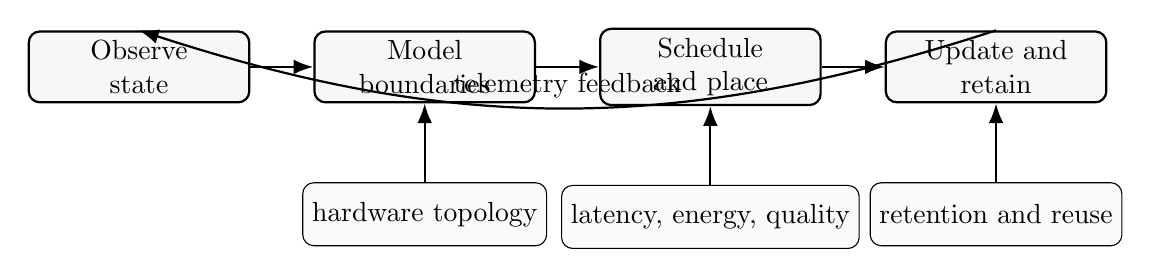
\begin{tikzpicture}[
  node distance=9mm and 8mm,
  block/.style={draw, rounded corners, thick, align=center, minimum width=28mm, minimum height=9mm, fill=black!3},
  side/.style={draw, rounded corners, align=center, minimum width=24mm, minimum height=8mm, fill=black!2},
  arrow/.style={-{Latex[length=2.5mm]}, thick}
]
\node[block] (observe) {Observe\\state};
\node[block, right=of observe] (model) {Model\\boundaries};
\node[block, right=of model] (schedule) {Schedule\\and place};
\node[block, right=of schedule] (update) {Update and\\retain};

\draw[arrow] (observe) -- (model);
\draw[arrow] (model) -- (schedule);
\draw[arrow] (schedule) -- (update);
\draw[arrow, bend left=18] (update.north) to node[above] {telemetry feedback} (observe.north);

\node[side, below=10mm of model] (hardware) {hardware topology};
\node[side, below=10mm of schedule] (service) {latency, energy, quality};
\node[side, below=10mm of update] (memory) {retention and reuse};

\draw[arrow] (hardware.north) -- (model.south);
\draw[arrow] (service.north) -- (schedule.south);
\draw[arrow] (memory.north) -- (update.south);
\end{tikzpicture}

\caption{Integrated runtime loop for future stateful infrastructure. Observation, boundary modeling, scheduling, and update control should be coupled rather than deployed as isolated policies.}
\label{fig:runtime-loop}
\end{figure*}

\subsection{Evaluation Dimensions for Future Surveys and Systems}

An enduring weakness of the area is evaluation fragmentation. Access papers often report throughput and contention reduction, execution papers report speedup or energy savings, and evolution papers report quality or forgetting. These are all important, but they make it hard to compare whether two systems are solving the same problem at different phases of the loop or genuinely addressing different control surfaces. A more coherent evaluation vocabulary should at least track four dimensions.

The first dimension is \emph{steady-state efficiency}, including throughput, amortized cost per useful result, and locality-sensitive resource use. The second is \emph{tail behavior}, including percentile latency, burst amplification, and recovery delay. The third is \emph{state quality}, including bounded approximation error, retrieval quality under drift, and retention value under memory budgets. The fourth is \emph{operational sustainability}, including migration cost, update overhead, and how quickly a control loop re-stabilizes after workload or hardware changes. Systems that score well on only one dimension can still be valuable, but they should be described as local improvements rather than full state-management solutions.

For survey authors, this evaluation vocabulary provides a way to compare systems without flattening their contributions. A streaming scheduler and a dynamic retriever may report different headline metrics, yet both can be judged by whether they expose a stable state object, define an optimization boundary around it, and connect local policy decisions to long-horizon system behavior. That comparability is one reason the state-management perspective is useful beyond any single subcommunity.

\subsection{A Design Space for Stateful Runtime Architectures}

The previous sections reviewed mechanisms by topic. This section restructures the same knowledge as a practical architecture design space. The goal is to make explicit which design decisions tend to co-travel in successful systems and which combinations repeatedly cause fragility. We focus on four architectural axes: state granularity, control-plane coupling, lifecycle management, and service-boundary alignment.

\subsubsection{State Granularity: Record, Key, Segment, and Session}

A first architectural choice is the granularity at which state is represented and controlled. Record-level granularity offers maximal flexibility but often suffers from high metadata overhead and weak locality. Key-level granularity, common in stream processing, can align naturally with partitioning and migration but can become skew-prone under hot keys~\cite{zhang2019briskstream,mao2025spacker}. Segment- or page-level granularity, prominent in modern LLM serving, trades finer control for stronger packing and transfer efficiency in memory-bound paths~\cite{kwon2023pagedattention,agrawal2024sarathi}. Session- or conversation-level granularity, common in agentic and retrieval-heavy systems, simplifies policy interfaces but can hide substantial internal heterogeneity in reuse value and retention cost~\cite{zheng2023sglang,wang2024hipporag}.

The most robust systems usually support more than one granularity and explicitly model conversion cost between them. For instance, a runtime may collect telemetry at key-level but schedule migration at chunk-level, or retain retrieval memory at document-level while serving lookups at token-level interaction granularity~\cite{khattab2020colbert}. A recurring failure mode is locking the entire system into one granularity because an early implementation made it convenient. That shortcut often appears efficient at prototype scale, then becomes a hard scalability ceiling once workloads diversify.

\subsubsection{Control-Plane Coupling: Embedded, Sidecar, or Shared Service}

A second choice is where state control logic lives. Embedded control keeps policy decisions near execution and can minimize coordination latency. However, it often creates fragmented policy semantics across subsystems. Sidecar-style control improves modularity and operability but can introduce lag between telemetry and action if the sidecar does not receive sufficiently rich state-change signals. Shared memory-control services offer stronger global consistency and reuse across workloads, yet risk becoming bottlenecks unless their APIs are designed around coarse enough operations and composable intents.

Historical systems illustrate each tradeoff. Stream engines with deeply embedded scheduling and state-placement logic can react quickly to contention but often need substantial refactoring when recovery and migration policies evolve~\cite{zhang2020concurrent,zhao2024recovery}. Serving systems that elevate memory control (for example, KV paging or phase-aware admission) to clearer runtime layers gain better policy visibility but must invest more in interface stability and backpressure semantics~\cite{kwon2023pagedattention,agrawal2024sarathi,holmes2024fastgen}. Retrieval-memory stacks frequently begin with loosely coupled indexing services, then move toward tighter control-plane integration once update cadence and quality drift become dominant concerns~\cite{karpukhin2020dpr,zhang2026flowrag}.

\subsubsection{Lifecycle Management: Admit, Place, Mutate, Compact, Evict}

Stateful runtime design is often framed around placement only. In practice, robust systems require an explicit lifecycle pipeline with at least five stages: admission, placement, mutation, compaction, and eviction. Admission controls whether new state should enter the active working set. Placement decides where it resides relative to compute paths. Mutation governs update semantics and write amplification. Compaction controls structural debt accumulated by updates and deletions. Eviction determines which state leaves the active tier and under what quality or recovery constraints.

This lifecycle framing unifies otherwise separate communities. In stream processing, admission can correspond to which keys or windows are promoted into fast paths; mutation corresponds to incremental state update and checkpoint integration; compaction appears in state backend maintenance and log trimming. In LLM serving, admission maps to request acceptance under memory pressure; placement maps to KV page residency; mutation maps to decode-time growth and prefix-share edits; compaction and eviction appear as memory reclamation and reuse-window tuning. In retrieval systems, admission maps to indexing policy under dynamic corpora; placement maps to tiered vector storage; mutation maps to embedding refresh and graph rewiring; compaction maps to index maintenance; eviction maps to stale-memory retirement.

When any one stage is implicit, systems become difficult to reason about under stress. For example, if compaction policy is absent from the design model, mutation cost can silently dominate over time and negate throughput gains that were visible in short benchmarks. Similarly, if admission is treated as an outer load-shedding mechanism rather than a first-class state policy, latency can remain unstable even after aggressive scheduling optimizations.

\subsubsection{Service-Boundary Alignment: Local Wins vs End-to-End Wins}

A final architectural axis is alignment between local optimization targets and user-facing service boundaries. Many papers report local speedups that are real but operationally fragile because they optimize inside an unmodeled boundary. Boundary-aware systems are explicit about what is held fixed (latency percentile, quality floor, recovery objective) and what is allowed to move (throughput, energy, memory footprint). This distinction is central in approximation-aware systems~\cite{zeng2024pecj,zeng2024libamm}, memory-bound serving runtimes~\cite{gujarati2020clockwork,kwon2023pagedattention}, and dynamic retrieval stacks where quality drift accumulates over time~\cite{asai2024selfrag,wang2024hipporag}.

For practitioners, the immediate implication is that architecture reviews should require a written boundary contract for each state mechanism: which service metric it claims to improve, under which workload assumptions, and with what fallback behavior when assumptions fail. Absent this contract, integration teams tend to inherit brittle local optimizations with unclear operational envelopes.

\subsection{Failure Modes and Anti-Patterns}

Survey papers often focus on successful mechanisms and under-discuss recurring anti-patterns. An explicit anti-pattern taxonomy is useful because it transforms "what to avoid" into a reusable review checklist.

\subsubsection{Telemetry-Action Mismatch}

A common failure is collecting state metrics that cannot trigger actionable runtime decisions. Systems may expose queue lengths, cache usage, or retrieval hit rates, but if these signals are not mapped to explicit control actions (for example, repartitioning, phase splitting, retention resizing), they become dashboard artifacts rather than control inputs. Telemetry quality should be judged by actionability and latency, not by cardinality of exported metrics.

\subsubsection{Policy Layering Without Conflict Semantics}

Another anti-pattern is policy accretion without conflict resolution. Teams add contention mitigation, then add migration heuristics, then add quality guards, each locally justified. Without explicit precedence or composition semantics, the resulting policy stack can oscillate or deadlock. This appears across stream scheduling, serving admission, and retrieval-update control. Systems that remain stable generally encode a hierarchy (hard constraints, soft objectives, tie-breakers) rather than a flat set of reactive rules.

\subsubsection{One-Shot Benchmarking of Non-Stationary Mechanisms}

Many state mechanisms are fundamentally temporal, yet are evaluated on short stationary runs. This mismatch is particularly harmful for retention and retrieval policies where degradation appears only after update cycles~\cite{zhou2025ferret,zhang2026flowrag}. Robust evaluation should include warmup, disturbance, adaptation, and re-stabilization phases. Otherwise, papers can overstate improvements that disappear under drift.

\subsubsection{Ignoring Write Amplification in "Read-Optimized" Designs}

Read-side acceleration often hides expensive write-side debt. Dense retrieval indexes, long-context memory stores, and incremental stream summaries can all accumulate maintenance overhead that is invisible in read-focused benchmarks. A mechanism should not be considered efficient if it simply externalizes cost into deferred compaction, index rebuild, or retraining windows.

\subsubsection{Treating State Ownership as Static}

Ownership assumptions that are valid at small scale often fail under bursty multi-tenant workloads. Static ownership models impede migration, sharing, and reclamation, and complicate fault recovery. Designs that explicitly represent transferable ownership and bounded lease semantics tend to adapt better under dynamic pressure, although they require stronger correctness reasoning.

\subsection{A Systems Blueprint for Building Stateful Infrastructure}

This section converts the survey into an implementation-oriented blueprint. The intent is not to prescribe one architecture, but to provide a minimally complete set of components and contracts that can be specialized by domain.

\subsubsection{Blueprint Layer 1: State Catalog and Schema Contracts}

Every production runtime should begin with a machine-readable state catalog: state object names, granularity, mutability class, lifecycle stage, and quality sensitivity. This catalog can be seen as a control-plane schema for runtime state. Without it, policy modules rely on implicit assumptions that quickly diverge across teams.

For survey continuity, authors can map each reviewed system into this catalog format. Doing so exposes where papers are comparable and where they solve fundamentally different state problems. It also helps identify under-specified designs that report strong results without clear state typing.

\subsubsection{Blueprint Layer 2: Observation and Disturbance Detection}

Observation should include both steady metrics and disturbance indicators. Steady metrics capture normal load and quality behavior; disturbance indicators detect shifts such as hotspot flips, phase imbalance, retrieval drift, or memory-fragmentation spikes. Disturbance-aware control loops are essential for systems whose workload phases differ sharply, as in prefill/decode serving or periodic retriever refresh.

An effective observation layer should expose confidence and delay metadata for each signal. Control policies that treat delayed telemetry as current truth are a major source of oscillation. Survey authors should document this explicitly when summarizing papers with online control claims.

\subsubsection{Blueprint Layer 3: Boundary Model and Decision Kernel}

The decision kernel should consume state catalog and observation streams to build boundary-aware decisions. A useful abstraction is a constrained optimizer with two classes of inputs: hard constraints (SLA, quality floor, memory limit) and soft objectives (throughput, energy efficiency, migration overhead). The kernel can be heuristic, model-based, or learned, but it should always produce auditable decisions and confidence estimates.

For systems papers, this is where many contributions differ: some improve signal quality, some improve model accuracy, some improve solver latency, and some improve safety under uncertainty. Presenting those differences through one decision-kernel abstraction makes cross-paper comparison much cleaner.

\subsubsection{Blueprint Layer 4: Actuation Interfaces}

Actuation interfaces should be explicit and idempotent where possible. Typical actions include repartition, migrate, remap, resize memory tier, adjust admission threshold, trigger compaction, or change retention window. Idempotence and bounded rollback are important because control loops may reissue actions under noisy telemetry.

Systems that expose only monolithic reconfiguration APIs tend to react too slowly under real-time pressure. Fine-grained actuation paths improve responsiveness but require careful conflict handling when multiple policies target overlapping state objects.

\subsubsection{Blueprint Layer 5: Safety and Recovery Envelope}

A stateful system is incomplete without an explicit safety envelope: invariants that must hold during and after control actions. Examples include bounded replay lag, consistency constraints on shared indexes, or no-eviction sets during critical decode windows. Recovery should be integrated into the same envelope, not treated as a separate mode.

The survey literature repeatedly suggests that performance and recovery cannot be cleanly separated once state is dynamic~\cite{chandy1985snapshot,schneider1990state,zhao2024recovery}. Blueprint implementations should therefore evaluate control actions against both steady-state and recovery invariants.

\subsection{Cross-Domain Case Studies}

To make the framework concrete, we provide three cross-domain case studies. Each case maps a practical scenario to the scaffold and blueprint described above.

\subsubsection{Case Study A: Multi-Tenant LLM Serving with Burst Arrival}

\textbf{Scenario.} A serving cluster handles mixed prompt lengths, intermittent bursts, and strict p99 latency targets. The runtime currently uses static batching and simple memory caps.

\textbf{State objects.} KV pages, prefix-share indexes, request queues, phase-specific occupancy traces.

\textbf{Control surfaces.} Admission thresholding, phase-aware scheduling, page placement, prefix-share windowing, reclamation timing.

\textbf{Coupling path.} Burst arrivals increase admission pressure, which increases decode-phase queueing, which increases KV growth and memory pressure, which then feeds back into reduced effective batching and degraded tail latency.

\textbf{Boundary model.} Hard constraints: p99 latency and memory safety. Soft objective: maximize stable throughput. Disturbance signal: phase imbalance and fragmentation slope.

\textbf{Expected lessons.} Improvements come less from one faster kernel and more from coherent lifecycle control of short-lived state~\cite{kwon2023pagedattention,agrawal2024sarathi,holmes2024fastgen}. Policies that optimize only allocation or only scheduling tend to plateau early.

\subsubsection{Case Study B: Stateful Stream Processing Under Reconfiguration}

\textbf{Scenario.} A stream engine must scale out during bursts and recover quickly from worker failure while maintaining bounded latency.

\textbf{State objects.} keyed windows, operator state shards, migration logs, checkpoint metadata.

\textbf{Control surfaces.} migration grain, trigger policy, replication factor, checkpoint cadence, replay window.

\textbf{Coupling path.} Reconfiguration decisions alter locality and transfer volume; recovery policies alter log pressure; both affect future contention and scheduling.

\textbf{Boundary model.} Hard constraints: correctness and recovery objective. Soft objective: minimize latency amplification during migration.

\textbf{Expected lessons.} Treating elasticity and fault handling as shared state-transfer problems yields better stability than implementing them as separate subsystems~\cite{nasir2019megaphone,fernandez2013osm,zhao2024recovery}.

\subsubsection{Case Study C: Retrieval Memory with Continuous Corpus Drift}

\textbf{Scenario.} A RAG service ingests frequent content updates and must preserve answer quality without full index rebuilds.

\textbf{State objects.} vector index, late-interaction caches, graph memory, retention metadata.

\textbf{Control surfaces.} incremental indexing policy, refresh cadence, compaction schedule, stale-memory eviction.

\textbf{Coupling path.} Aggressive updates improve freshness but can destabilize retrieval quality and query latency due to index churn.

\textbf{Boundary model.} Hard constraints: quality floor and uptime. Soft objective: reduce amortized update cost.

\textbf{Expected lessons.} Retrieval quality and system cost should be evaluated jointly across long horizons; short static evaluations understate lifecycle debt~\cite{karpukhin2020dpr,khattab2020colbert,wang2024hipporag,zhang2026flowrag}.

\subsection{Methodological Notes on Survey Synthesis}

To keep cross-domain synthesis coherent, we use a consistent integration protocol.

\paragraph{Step 1: Paper Intake and Typing}

Each candidate paper should be typed by state object, control surface, and boundary metric before prose integration. Papers that cannot be typed should remain in a backlog list until clarified.

\paragraph{Step 2: Mechanism Grouping Before Writing}

Papers should be grouped by mechanism family, not venue chronology. Typical families include migration control, memory reclamation, phase-aware scheduling, retrieval index maintenance, and quality-bounded approximation.

\paragraph{Step 3: Comparative Paragraph Minimum}

A subsection extension should contain at least one comparative paragraph that contrasts two or more mechanisms under a shared boundary. Purely additive summaries are insufficient for a survey article targeting CSUR standards.

\paragraph{Step 4: Gap Statement and Testable Claim}

Every new subsection should end with a gap statement and one testable systems claim. This ensures the survey remains analytically forward-looking rather than encyclopedic.

\paragraph{Step 5: Reproducibility Checks}

Before accepting new content, authors should verify citation resolution, terminology consistency, and section-level boundary clarity. A practical checklist is: (1) no undefined references, (2) no duplicate concept aliases without mapping, (3) each paragraph ties mechanism to boundary.

\subsection{Analytical Maturity}

\subsubsection{Cross-Layer Mechanism Synthesis}

Across access, execution, and evolution, the literature shows a shared systems pattern: local policy gains often disappear once effects propagate through the state lifecycle. In streaming systems, fine-grained synchronization and partitioning can improve multicore scalability~\cite{zhang2017revisiting,zhang2020concurrent}, yet these gains degrade when topology and locality are not co-optimized~\cite{zhang2019briskstream}. Hardware-conscious lines similarly show that movement and representation of state can dominate kernel-level arithmetic gains~\cite{zhang2020finestream,zeng2024cstream}.

Inference runtimes exhibit the same mechanism. Paged KV management and reuse-aware serving turn memory from an implementation detail into an explicit control object~\cite{kwon2023pagedattention,zheng2023sglang}. However, allocator improvements alone are insufficient when phase asymmetry between prefill and decode remains unscheduled~\cite{agrawal2024sarathi,holmes2024fastgen}. This mirrors transactional stream findings where stable behavior requires dependency-aware online control rather than static plans~\cite{mao2023morphstream}.

Approximation and retrieval lines reinforce boundary-first design. Approximate kernels and compensation mechanisms are sustainable only when quality floors are integrated into runtime decisions~\cite{zeng2024pecj,zeng2024libamm}. In long-horizon retrieval and retention systems, update and maintenance policies directly shape downstream quality-cost trajectories~\cite{zhou2025ferret,zhang2026flowrag}. Without explicit boundary models, systems accumulate maintenance debt that later erases short-run gains.

Recovery and elasticity also converge into one state-transfer problem. Snapshotting, migration, and recovery acceleration are most robust when they share transfer semantics and observability channels instead of being isolated subsystems~\cite{carbone2015asynchronous,fernandez2013osm,zhao2024recovery}. This suggests a unified control-plane abstraction for ownership transfer across steady-state and failure-time operation.

The strongest cross-domain principle is therefore state-as-scheduling-object. Instead of scheduling tasks over passive data, modern runtimes schedule around mutable state objects (KV pages, operator shards, retrieval structures, retention buffers), and then map compute accordingly~\cite{zheng2023sglang,zhong2024distserve,patel2024splitwise}. Explicit lifecycle stages (admit, place, mutate, compact, reclaim) make closed-loop governance feasible.

Persistent unresolved mechanism gaps include:
\begin{enumerate}[leftmargin=*]
\item high-fidelity observability for semantic state conflicts beyond coarse counters;
\item cross-tier lifecycle coordination for short-lived and long-lived memory objects;
\item policy-composition semantics that prevent oscillation under overlapping triggers;
\item long-horizon accounting of maintenance debt and reuse-value decay.
\end{enumerate}

\subsubsection{Evaluation Protocols and Threats to Validity}

Evaluation should treat state management as closed-loop control, not isolated optimization. Each experiment should explicitly specify the state object, control surface, and service boundary before reporting outcomes. This prevents local speedups from being misread as end-to-end gains when lifecycle paths remain unchanged~\cite{kwon2023pagedattention,agrawal2024sarathi,zheng2023sglang,mao2023morphstream}.

Disturbance-driven evaluation is required. Stationary replay alone hides instability that appears under burst, skew, and phase transitions. Protocols should fix random seeds, preserve disturbance timestamps, and report both phase-local and aggregate outcomes so inflection points are auditable~\cite{zhang2019briskstream,zhang2020concurrent}.

A minimal protocol suite should include:
\begin{enumerate}[leftmargin=*]
\item \textbf{burst disturbance}: short high-intensity arrivals stressing fragmentation and queue growth;
\item \textbf{skew disturbance}: popularity flips testing migration and reuse stability;
\item \textbf{topology disturbance}: controlled device/NUMA perturbations isolating movement sensitivity;
\item \textbf{semantic disturbance}: update drift probing retention and index-evolution coupling.
\end{enumerate}

Long-horizon metrics are necessary when claims involve reuse or adaptation: reuse survival, reclamation debt, update-to-benefit lag, post-shock recovery half-life, and quality-retention trajectories. These reveal delayed regressions that short-window throughput cannot capture~\cite{kwon2023pagedattention,zhou2025ferret,zhang2026flowrag}.

Coupling-aware ablations should be standard. Components must be evaluated not only marginally but also under interaction terms (access-only, execution-only, evolution-only, joint), because many gains emerge only when controls are coordinated~\cite{mao2023morphstream,zeng2024cstream,zeng2024pecj}.

Negative results should be first-class evidence. Reports should include boundary failures, sign reversals (for example, higher reuse but worse p99), and oscillation windows under disturbance. This avoids survivorship bias and tightens claim scope to measured envelopes~\cite{zhang2020concurrent,zeng2024pecj,wu2023sentistream}.

Threats to validity should be operationalized as constraints: internal validity via seed/time control and warmup policy; construct validity via strict separation of overlap opportunity vs realized reuse; external validity via multi-regime and topology-perturbed replication. Claims should remain bounded to tested disturbance and lifecycle horizons.

\subsubsection{Research Agenda Beyond Isolated Policy Tuning}

The next stage of progress is architectural rather than heuristic: state must become the central abstraction across streaming, serving, retrieval, and retention systems. Isolated policy tuning can improve local regimes, but cross-layer instability persists when lifecycle governance is fragmented~\cite{zhang2019briskstream,mao2023morphstream,kwon2023pagedattention,agrawal2024sarathi}.

First, future runtimes need unified state-lifecycle observability that links low-level contention with service-level quality drift~\cite{zhang2017revisiting,zhang2020concurrent,zhang2026flowrag}. Without path-level telemetry, controllers cannot estimate deferred costs created by current decisions.

Second, state-centric scheduling should supersede task-centric scheduling on heterogeneous hardware. Placement, phase control, and quality-bounded approximation must be coordinated over one state-transition graph that includes compute and memory tiers~\cite{agrawal2024sarathi,zhong2024distserve,zeng2024pecj,zeng2024libamm}.

Third, memory middleware is needed for dynamic AI services. Existing methods provide strong model-centric mechanisms but weak shared systems interfaces for admission, retention, refresh, and compaction across ephemeral and persistent memory objects~\cite{kirkpatrick2017ewc,lopez2017gem,guu2020realm,lewis2020rag,wang2024hipporag}.

Fourth, recovery semantics should be integrated into steady-state control. Throughput-oriented mutation and placement decisions must be constrained by explicit recovery-time envelopes so optimization does not accumulate unrecoverable state debt~\cite{carbone2015asynchronous,fernandez2013osm,zhao2024recovery}.

Fifth, the community needs policy-composition semantics. As controllers for compression, reuse, quality bounds, and admission accumulate, precedence and conflict resolution must be formalized to prevent oscillation under non-stationary load~\cite{zeng2024cstream,zeng2024pecj,zheng2023sglang}.

Finally, benchmark norms should shift from short-run peak gains to lifecycle stability under disturbance and drift, including explicit negative/neutral outcomes and maintenance-debt accounting~\cite{wang2026candor,zhou2025ferret}. This transition from isolated mechanisms to integrated governance is the most direct path toward robust stateful infrastructure.

\subsection{Cross-Domain Comparative Synthesis}

This section deepens the survey with domain-specific comparative maps. Each map answers the same three questions: which state object dominates in the domain, which runtime controls are mature, and which control seams remain under-developed.

\subsubsection{Map I: Streaming and Transactional Dataflows}

Streaming and transactional dataflow systems share a core tension: they want low-latency updates over mutable shared state while preserving deterministic recovery and bounded operational overhead. From early stream engines to modern transactional stream processors, the visible progress has largely come from making state transitions explicit in the runtime rather than hidden in operator code paths~\cite{abadi2003aurora,murray2013naiad,mao2023morphstream}.

A first mature control seam is access topology. Systems that explicitly reason about locality, key skew, and synchronization surfaces achieve more stable behavior than those optimizing only per-operator throughput~\cite{zhang2019briskstream,zhang2020concurrent}. The key lesson is that contention and locality are endogenous: scheduling decisions reshape them, and measurement must feed back into scheduling.

A second mature seam is recovery coupling. Recovery is no longer a pure failure-mode concern; it is a steady-state design partner. Checkpoint cadence, log granularity, and migration mechanism together define whether latency remains bounded during faults and reconfiguration~\cite{carbone2015asynchronous,zhao2024recovery}. Systems that isolate these concerns administratively often pay duplicated state-transfer overhead.

A third seam is elasticity with state ownership transfer. The best-known failure mode is scaling compute capacity without designing explicit ownership transfer contracts for state. Elasticity then appears successful in microbenchmarks but unstable in long-running mixed workloads. Operator-state-management lines make this tradeoff visible and suggest that scale-out and fault tolerance should share a common state-transfer substrate~\cite{fernandez2013osm,nasir2019megaphone}.

Open gaps remain significant. Most systems still under-model multi-tenant interference where contention surfaces change with tenant mix rather than input rate alone. Another recurring gap is weak support for semantic state objects (for example, dynamic retrieval caches in stream-adjacent applications), where access conflicts are not purely key-based and cannot be managed by partitioning alone.

\subsubsection{Map II: Hardware-Conscious and Approximate Stateful Execution}

Hardware-conscious systems established that stateful efficiency depends on movement and representation choices as much as arithmetic intensity. Fine-grained CPU/GPU coordination, dictionary-aware processing, and compression-aware scheduling illustrate this shift~\cite{zhang2020finestream,zeng2024cstream}. The domain's strongest contributions expose state representation as a runtime control surface rather than a static storage decision.

Approximation-aware systems add a boundary model that is still underused outside their subcommunity. Mechanisms such as proactive compensation, adaptive sampling, and approximate matrix kernels are valuable because they couple quality boundaries to runtime cost decisions~\cite{zeng2024pecj,tang2025freesam,zeng2024libamm}. Without this coupling, approximation can improve local throughput while degrading user-level utility.

The map suggests two cross-domain lessons. First, state representation should be treated as a dynamic control variable (switchable compression level, adaptive summary fidelity, selective decompression path) rather than a compile-time parameter. Second, quality budgets must be first-class citizens in scheduling, not post-hoc validation checks.

Open gaps include weak portability of policy tuning across hardware topologies and limited integration between approximation control and recovery semantics. A system may know how to bound error during normal operation but may not define what error contract holds during recovery or reconfiguration.

\subsubsection{Map III: LLM Serving and Short-Lived Memory Lifecycles}

LLM serving has made state-lifecycle management impossible to ignore. KV caches, prefix-sharing structures, and phase-skewed queues now dominate runtime behavior in many deployments~\cite{kwon2023pagedattention,agrawal2024sarathi}. This domain has progressed rapidly because it translated memory overhead into an explicit scheduling and admission problem rather than a hidden allocator concern.

One mature seam is memory layout and allocation policy. Paging-style approaches and explicit sharing surfaces improved memory efficiency and therefore expanded feasible batching regions~\cite{kwon2023pagedattention}. Another seam is phase-aware control: separating prefill and decode characteristics exposes different bottlenecks and enables targeted scheduling and placement actions~\cite{agrawal2024sarathi,zhong2024distserve,patel2024splitwise}.

Structured-program serving adds a further layer: runtime-managed reuse boundaries across multi-call workflows, constrained decoding, and retrieval subcalls~\cite{zheng2023sglang}. In these settings, state lifecycle is no longer per-request only; it includes reusable intermediate objects whose value depends on program structure.

Open gaps include cross-node lifecycle coordination for short-lived state, benchmark protocols that cover disturbance phases (burst, warmup, drift), and principled integration between serving memory control and retrieval-memory updates. Most evaluations still optimize one layer at a time.

\subsubsection{Map IV: Retrieval Memory and Vector-Index State Layers}

Retrieval systems moved from lexical inverted indexes to dense and hybrid memory substrates where indexing, refresh, and serving are tightly coupled state problems~\cite{karpukhin2020dpr,khattab2020colbert}. The key architectural transition is from "querying documents" to "maintaining a living memory layer" with explicit update and compaction debt.

Dense dual-encoder systems improved retrieval quality and throughput tradeoffs, while late-interaction approaches preserved richer matching signals with manageable online cost by shifting computation between offline and online phases. Graph- and structure-enhanced memory approaches pushed the domain toward long-horizon memory models that better capture multi-hop and evolving knowledge dependencies~\cite{wang2024hipporag,sarthi2024raptor}.

For systems researchers, the central insight is that retrieval quality is a lifecycle property, not just a model property. Refresh cadence, index maintenance policy, and stale-memory eviction govern long-term quality-cost balance as strongly as encoder architecture.

Open gaps include unified treatment of dense, graph, and late-interaction memory objects in one control plane, and stronger operational metrics that connect index maintenance decisions to end-to-end service SLOs.

\subsubsection{Map V: Continual Learning and Retention Governance}

Continual-learning systems contribute a mature language for retention under bounded memory. Replay strategies, interference-aware selection, and constrained update rules formalize retention as a governed state problem~\cite{kirkpatrick2017ewc,lopez2017gem,aljundi2019mir}. This perspective is highly relevant to retrieval and serving systems that increasingly maintain evolving memory under strict resource constraints.

The strongest mechanisms explicitly optimize both near-term adaptation and long-term retention value. They avoid the simplistic recency heuristic and instead prioritize representativeness, interference control, or future utility. This is conceptually aligned with memory middleware goals in dynamic AI services.

Open gaps include system-level integration: many continual-learning methods remain model-centric and do not specify operational semantics for distributed retention stores, update fault handling, or cross-service consistency.

\subsubsection{Comparative Mechanism Matrices}

The following long-form matrices make cross-domain comparison explicit at scale and complement the narrative synthesis with structured side-by-side evidence.

\renewcommand{\arraystretch}{1.08}

\begin{longtable}{>{\raggedright\arraybackslash}p{0.16\textwidth}>{\raggedright\arraybackslash}p{0.2\textwidth}>{\raggedright\arraybackslash}p{0.2\textwidth}>{\raggedright\arraybackslash}p{0.2\textwidth}>{\raggedright\arraybackslash}p{0.18\textwidth}}
\caption{Large-scale mechanism matrix across representative papers.}\label{tab:large-matrix-a}\\
\toprule
Paper line & Dominant state object & Primary control surface & Evaluated boundary & Extension note \\
\midrule
\endfirsthead
\toprule
Paper line & Dominant state object & Primary control surface & Evaluated boundary & Extension note \\
\midrule
\endhead
Aurora/Borealis~\cite{abadi2003aurora,abadi2005borealis} & operator-local continuous-query state & operator graph management and adaptation & throughput/latency in streaming plans & extend with modern migration-control comparison \\
MillWheel/Naiad/Dataflow~\cite{akidau2013millwheel,murray2013naiad,akidau2015dataflow} & keyed windows and timely update state & event-time/state progression semantics & correctness-latency tradeoff & add reconfiguration stress protocol \\
BriskStream/Concurrent stream~\cite{zhang2019briskstream,zhang2020concurrent} & shared queues/indexes and synchronization state & topology-aware scheduling and partitioning & throughput under contention & include multi-tenant hot-key scenarios \\
MorphStream~\cite{mao2023morphstream} & transactional dependency state & online dependency-aware scheduling & latency/throughput stability & compare against static policy baselines \\
Fast recovery line~\cite{zhao2024recovery} & recovery metadata + logs & recovery-integrated control & recovery time + steady-state overhead & attach migration-recovery unification \\
Megaphone/OSM/SEEP~\cite{nasir2019megaphone,fernandez2013osm,fernandez2010seep} & movable operator-state shards & fine-grained migration and elasticity control & reconfiguration latency & add correctness envelope taxonomy \\
FineStream/CStream~\cite{zhang2020finestream,zeng2024cstream} & representation-aware operator state & hardware-conscious mapping + state path design & speed/energy-delay tradeoffs & extend to heterogeneous accelerator mixes \\
PECJ/LibAMM~\cite{zeng2024pecj,zeng2024libamm} & quality-sensitive intermediate state & approximation and compensation control & bounded quality vs cost & unify with service-level quality floors \\
vLLM~\cite{kwon2023pagedattention} & paged KV cache & allocation/sharing/reclamation policy & throughput at latency target & add cross-node lifecycle experiments \\
Sarathi-Serve~\cite{agrawal2024sarathi} & phase-skewed serving state & prefill/decode-aware scheduling & throughput-latency frontier & benchmark disturbance regimes \\
SGLang~\cite{zheng2023sglang} & reusable structured execution state & radix reuse + constrained decoding control & throughput on structured programs & map program-shape sensitivity \\
Clockwork/Clipper~\cite{gujarati2020clockwork,crankshaw2017clipper} & model/request serving state & predictability-driven dispatch and serving orchestration & tail-latency/SLO isolation & bridge to KV-era memory controls \\
DistServe/Splitwise/FastGen~\cite{zhong2024distserve,patel2024splitwise,holmes2024fastgen} & disaggregated phase state and queue state & phase split/disaggregation policy & goodput + tail behavior & integrate with admission governance \\
DPR/ColBERT~\cite{karpukhin2020dpr,khattab2020colbert} & dense and late-interaction retrieval indexes & offline/online retrieval decomposition & retrieval quality vs serving cost & add update/refresh lifecycle dimension \\
HippoRAG/FlowRAG~\cite{wang2024hipporag,zhang2026flowrag} & graph-enhanced and evolving retriever memory & dynamic memory evolution control & long-horizon quality and efficiency & add stale-memory debt metrics \\
Continual memory line~\cite{zhou2025ferret,li2026streamfp} & retained sample memory and selection traces & retention budgeting and selection policy & forgetting vs adaptation quality & connect with retrieval index retention \\
Approximate analytics line~\cite{agarwal2013blinkdb,goiri2015approxhadoop,chen2018incapprox} & summary/sample state & accuracy-cost budget control & latency/error boundaries & integrate with modern serving-style SLAs \\
Spanner/Calvin/FaRM line~\cite{corbett2012spanner,thomson2012calvin,dragojevic2014farm} & distributed transaction state and replication metadata & consistency/placement/concurrency control & correctness + latency + scale & compare with serving memory ownership models \\
CRDT and replicated-data line~\cite{shapiro2011crdt} & convergent replicated object state & conflict-free merge semantics & convergence and availability & study with retrieval-memory updates \\
\bottomrule
\end{longtable}

\begin{longtable}{>{\raggedright\arraybackslash}p{0.16\textwidth}>{\raggedright\arraybackslash}p{0.2\textwidth}>{\raggedright\arraybackslash}p{0.2\textwidth}>{\raggedright\arraybackslash}p{0.2\textwidth}>{\raggedright\arraybackslash}p{0.18\textwidth}}
\caption{Evaluation-and-gap matrix across representative state-management clusters.}\label{tab:large-matrix-b}\\
\toprule
Cluster & Recommended disturbance tests & Required metrics & Common blind spots & Open research direction \\
\midrule
\endfirsthead
\toprule
Cluster & Recommended disturbance tests & Required metrics & Common blind spots & Open research direction \\
\midrule
\endhead
State access under skew & hotspot flip, burst tenant switch, rebalance events & throughput, p99, conflict density, migration lag & stationary-load-only evaluation & add workload phase annotations to results \\
Recovery-integrated scheduling & fail-stop at different load phases, replay stress & recovery time, post-recovery stability, backlog clearance & treating recovery as isolated mode & quantify steady/recovery coupling cost \\
Elastic stream migration & scale-out/in under active joins/windows & migration overhead, latency amplification, ownership transfer delay & no ownership semantics during transfer & write ownership-state contract subsection \\
Hardware-conscious execution & topology perturbation and device contention & energy per useful result, latency, quality floor & microbenchmark-centric claims & add end-to-end boundary plots \\
Approximation control & drift + disorder injection & bounded error, utility loss, throughput & static error assumptions & evaluate adaptive error budgeting \\
KV cache lifecycle & long prompts + bursty decode + mixed sampling modes & memory waste, reuse ratio, p99, admission drop rate & allocator-only optimization view & add lifecycle-stage breakdown figures \\
Serving disaggregation & independent pressure on prefill/decode pools & goodput, queue imbalance, transfer overhead & homogeneous-request assumptions & build mixed-length benchmark suite \\
Structured serving programs & control-flow-heavy prompt programs & reuse hit rate, decode constraint overhead, tail latency & ignoring program-shape diversity & add program-template taxonomy \\
Retrieval index evolution & continuous corpus updates + stale data injection & recall@k, answer quality, update cost, query latency & one-shot index build assumption & define refresh-compaction schedules \\
Graph memory retrieval & multi-hop drift and conflicting evidence injection & quality robustness, latency, maintenance overhead & no maintenance debt accounting & add graph maintenance cost analysis \\
Continual retention policies & memory budget sweep with domain shift & forgetting, adaptation speed, retention overhead & model-only reporting without system costs & add retention-store systems metrics \\
Cross-domain middleware & concurrent serving + retrieval + update workloads & SLA violations, cross-layer backpressure, policy conflicts & layer-by-layer optimization & prototype unified control API discussion \\
Tiered memory architectures & hot/cold transition storms & promotion accuracy, movement cost, hit/miss latency gap & simplistic hotness heuristics & evaluate prediction-based tiering policies \\
Quality-bounded serving & quality floor shifts at runtime & quality, latency, throughput, fallback frequency & fixed-quality-threshold assumptions & add dynamic bound adaptation study \\
Scheduling-policy composition & overlapping policy triggers & oscillation frequency, convergence time, rollback count & no conflict semantics & define policy precedence model \\
Observability fidelity & delayed/noisy metrics simulation & decision regret, control delay, wrong-action rate & perfect telemetry assumption & add signal-confidence modeling subsection \\
Admission governance & adversarial burst and tenant unfairness workloads & admission fairness, SLA stability, rejection utility loss & average-only admission metrics & include per-tenant fairness analysis \\
Long-horizon reuse quality & week-scale synthetic drift phases & quality decay slope, refresh debt, maintenance spikes & short-run benchmark horizon & add multi-phase evaluation protocol \\
\bottomrule
\end{longtable}

\section{Conclusion}

This survey argued that state management is the unifying systems problem behind a wide range of modern runtimes. Whether the workload is transactional streaming, hardware-conscious analytics, or dynamic retrieval-augmented inference, the core challenges recur: making shared state observable, controlling access under concurrency, mapping execution onto complex hardware and service boundaries, and evolving memory without destabilizing future reuse.

The literature already provides strong ingredients for this agenda. Work on contention-aware access and scheduling established the observation-model-control chain for shared state. Hardware-conscious and quality-aware execution studies clarified why stable gains require joint modeling of topology, cost, and service boundaries. Recent work on online updates, continual retention, and dynamic retrieval showed that state evolution and reuse must be treated as first-class systems mechanisms. The key remaining step is integration: future systems should close the loop among access, execution, and evolution, turning state management into the central control plane of long-running services.

\begin{acks}
This draft was seeded from an academic-report storyline and a locally maintained publication archive, then reorganized into a survey taxonomy intended for ACM Computing Surveys. It should be treated as an evolving manuscript rather than a submission-ready version.
\end{acks}

\bibliographystyle{ACM-Reference-Format}
\bibliography{refs}

\end{document}